\documentclass[xcolor=dvipsnames]{beamer}

\usepackage{colortbl}
\usepackage{graphicx}
\usepackage{colortbl}
\usepackage{epstopdf}
\usepackage[export]{adjustbox}
\usepackage{caption}
\usepackage{amsmath}
\usepackage{mathtools}
\usetheme{Madrid}
\usepackage{url}
\usepackage{ulem, xpatch}
\usepackage{algorithm}
\usepackage{algorithmic}
\usepackage{arydshln}
%\usepackage{apacite}
\usepackage[backend=bibtex]{biblatex}
\renewcommand*{\bibfont}{\small}
\bibliography{mylit.bib}
%\renewcommand\bibliographytypesize{\footnotesize}

%\usepackage{caption}
%\usetheme{Rochester}
\usecolortheme[named=Purple]{structure}

\title[Data Analytics in Healthcare]{Data Analytics in Healthcare} 
\author[IEOR, IITB]{Arun R \\163190013 \\ \bigskip IE615: Data Analytics for Operations Research}

\newcommand{\spread}{\setlength{\itemsep}{\fill}}

\begin{document}
%\AtBeginSection[]
%{
%	\begin{frame}
%		\frametitle{Outline}
%		\tableofcontents[currentsection]
%	\end{frame}
%}

\begin{frame}
\titlepage
\end{frame}

\begin{frame}
	\frametitle{Outline}
	\tableofcontents
\end{frame}

\section{Introduction}
\begin{frame}{Introduction}
\begin{itemize}
\item The amount of data produced by healthcare industries grows exponentially. 
\item Bulk of the data comes from electronic health care, pharmacy, insurance claim, human tracking system and diagnostic instruments. 
\item The data can be leveraged using data analytics to provide better treatment to patients and reduce the operations cost. 
\item Healthcare data analytics can be used to,
\begin{itemize}
\item[--] \alert{Diagnose disease}
\item[--] Plan for disaster
\item[--] Understand patient flow
\item[--] Effectively manage resources and cost
\item[--] Reduce fraud  
\end{itemize} 
\end{itemize}
\end{frame}

\begin{frame}{Summary of Papers}
\begin{table}[]
\centering
\begin{tabular}{|l|l|l|}
\hline
Prediction           & Feature Selection                                                    & ML Algorithm                                                                                                     \\ \hline \hline
Breast Cancer        & F1-Score                                                             & SVM                                                                                                              \\ \hline
Diabetes             & \begin{tabular}[c]{@{}l@{}}Information Gain\\ and SMOTE\end{tabular} & \begin{tabular}[c]{@{}l@{}}Decision Trees,\\ Logistic Regression,\\ Naive Bayes and\\ Random Forest\end{tabular} \\ \hline
Hospital Readmission & Oversampling                                                         & \begin{tabular}[c]{@{}l@{}}Particle Swarm \\ Optimization based SVM\end{tabular}                                 \\ \hline
\alert{Breast Cancer}        & \alert{K-Means}                                                              & \alert{SVM}                                                                                                             \\ \hline
\end{tabular}
\end{table}
\end{frame}

\section{Breast Cancer Diagnosis: Problem Statement}
\begin{frame}{Problem Statement}
\begin{itemize}
\spread
\item To diagnose breast cancer using machine learning techniques.
\item Need a prediction model which is accurate and quick to build.  
\item Extract features from a given dataset using K-means clustering.
\item Build a SVM-based prediction model on the extracted features. 
\end{itemize}
\end{frame}

\section{Dataset}
\begin{frame}{Dataset: Instances}
\begin{itemize}
\spread
\item Name: Wisconsin Diagnostic Breast Cancer (WDBC) dataset
\item Date: November, 1965
\item Number of instances: 569
\item Number of instances in \textit{benign tumor} class: 357
\item Number of instances in \textit{malignant tumor} class: 212
\end{itemize}
\end{frame}

\begin{frame}{Dataset: Features}
\begin{itemize}
\spread
\item Number of features: 30
\item The features can be categorized as,
\begin{itemize}
\item[--] Radius
\item[--] Texture
\item[--] Perimeter
\item[--] Area
\item[--] Smoothness
\item[--] Compactness
\item[--] Concavity
\item[--] Concave points
\item[--] Symmetry
\item[--] Fractal Dimension
\end{itemize}
\item Mean, standard error and largest value are reported for each category.
\end{itemize}
\end{frame}

\begin{frame}{Notation and Definition}
K-means clustering is used to extract new features from the dataset. Notations used in this work are,
 
\begin{table}[H]
\centering
\begin{tabular}{|l|l|}
\hline
Notation      & Definition                                   \\ \hline
$K$           & Number of clusters                           \\
$F$           & Number of features in original dataset       \\
$N$			  & Number of instances							 \\	
$S_c$/$S_k$   & Set of points in $c^{th}$/$k^{th}$ cluster   \\
$X^i$         & $i^{th}$ input in dataset                    \\
$X^i_j$       & $j^{th}$ feature in $i^{th}$ input           \\
$X^{\mu_k}$   & Center of $k^{th}$ cluster                     \\
$X^{\mu_k}_j$ & $j^{th}$ feature of center of $k^{th}$ cluster \\ \hline
\end{tabular}
\end{table}
\end{frame}

\section{Feature Extraction and SVM Model}
\begin{frame}{Feature Extraction}
\begin{itemize}
\item K-means clustering is used to find hidden patterns in each class.
\item Cluster centers are used to extract new features.
\item Validity ratio is used to fix the number of clusters in each class. 
\end{itemize}
\begin{equation*}
\text{Validity Ratio} = \frac{d_{avg}}{d_{min}}
\end{equation*}
\hspace{1cm}where,
\begin{align*}
d_{avg} &= \displaystyle \frac{\sum_{k=1}^K \sum_{i \in S_k} \sqrt{\sum_{j=1}^F \big(X_j^i - X_j^{\mu_k}\big)}}{N}\\
d_{min} &= \min \bigg[\sum_{j=1}^F\sqrt{\big(X_j^{\mu_{k_2}} - X_j^{\mu_{k_2}}\big)^2}\bigg] \; \forall k_1 \neq k_2
\end{align*} 
\end{frame}

\begin{frame}{Original Results}
\begin{figure}[H]
  \begin{center}
    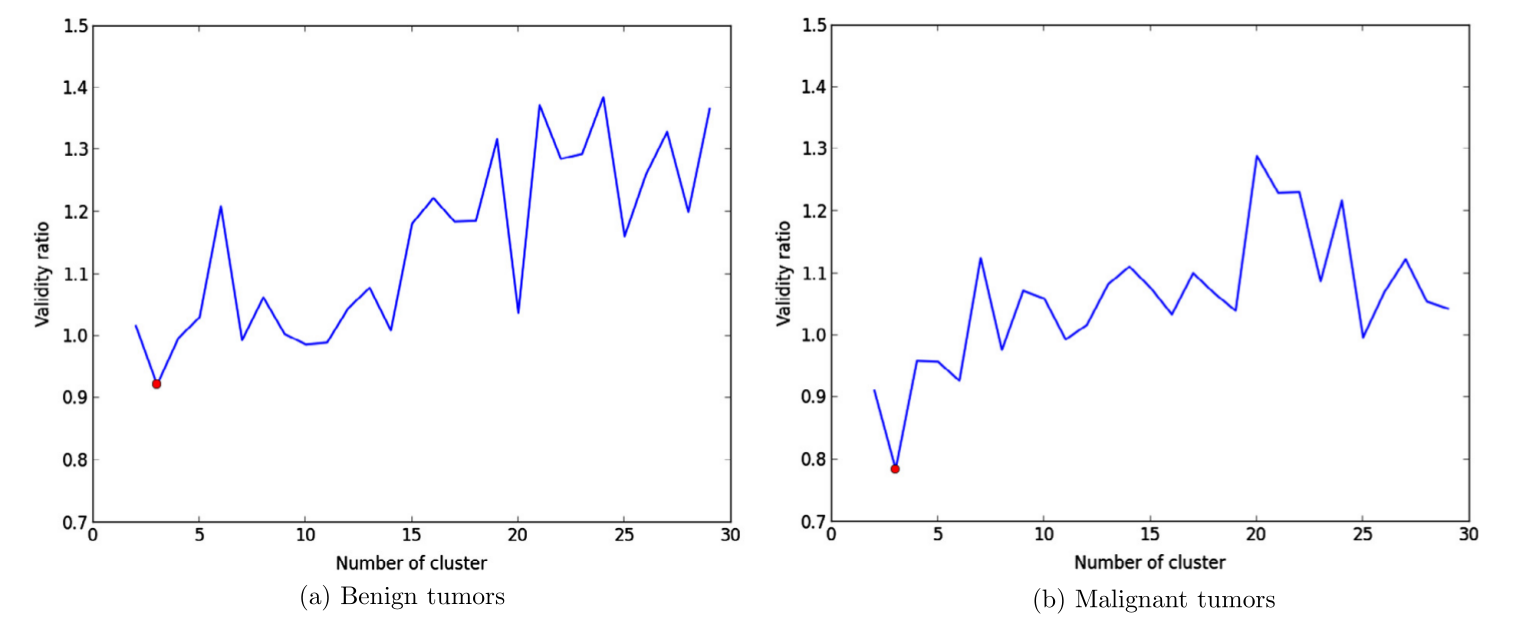
\includegraphics[scale=0.2]{Figures/BenignMalignantOriginal}
	%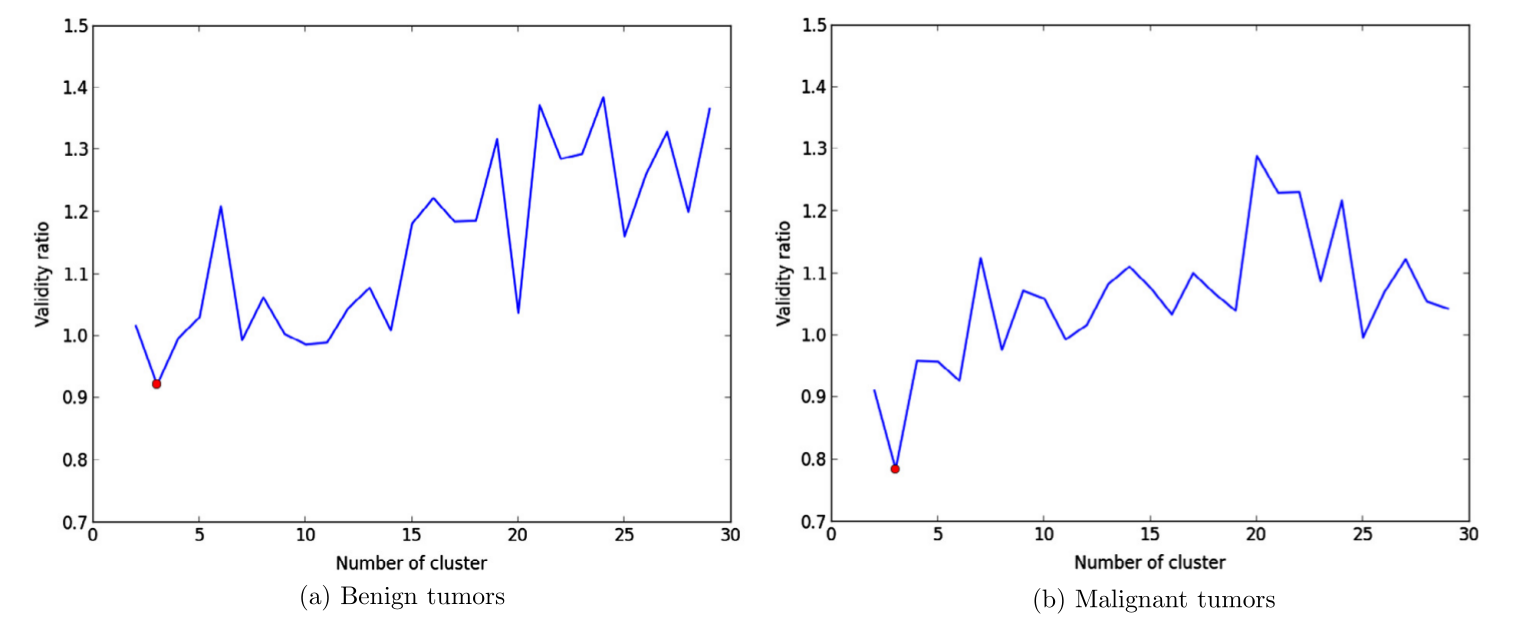
\includegraphics[trim={0cm 0.5cm 0cm 7cm},clip,scale=0.47]{Figures/BenignMalignantOriginal}  
  \end{center}
  %\vspace{-0.7cm}
  \caption{Variation of validity ratio with number of clusters}
\end{figure}

Optimal number of clusters is \alert{three} for both the classes.
\end{frame}

\begin{frame}{New Results (Benign): Full Normalization}
Instances of both the classes are normalized together.
\begin{figure}[H]
\begin{minipage}[t]{0.5\linewidth}
    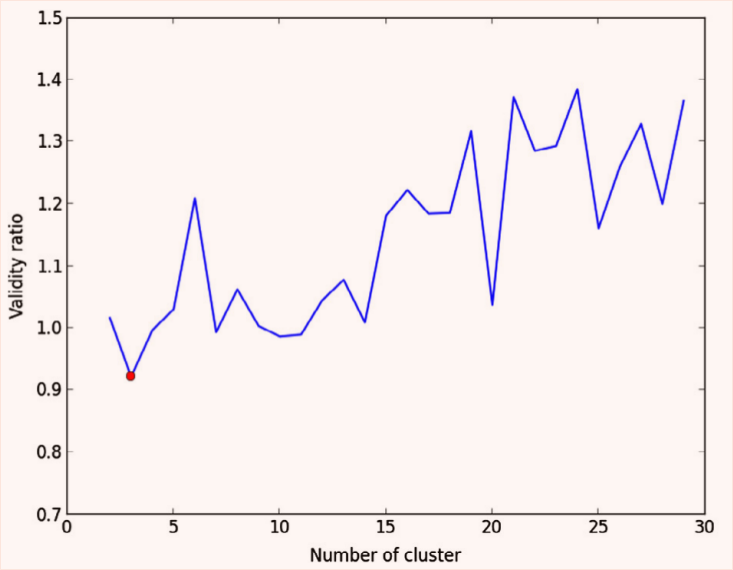
\includegraphics[scale=0.2]{Figures/BenignOriginal}
    \caption*{(a) Original Result}
\end{minipage}%
\begin{minipage}[t]{0.5\linewidth}
    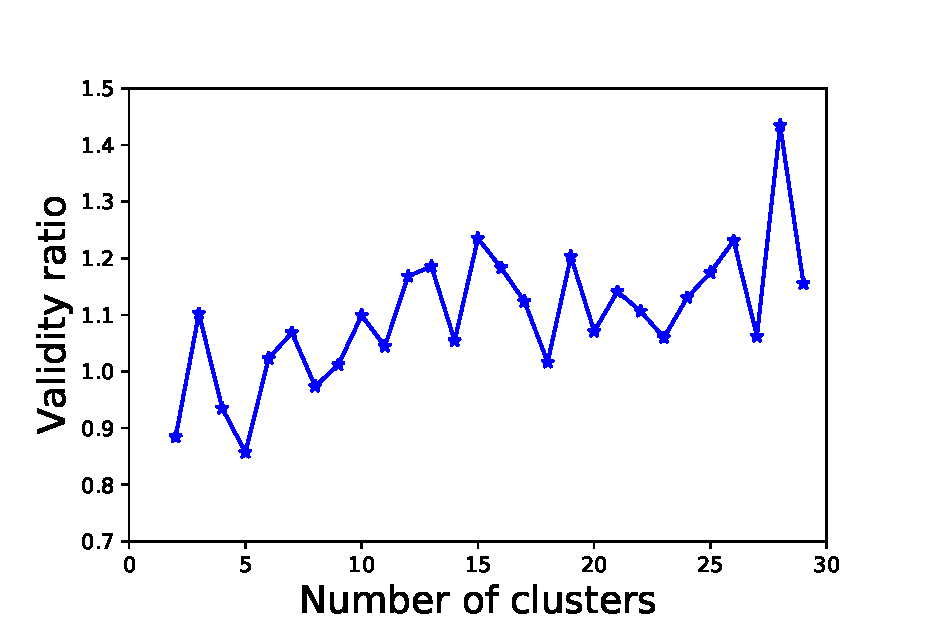
\includegraphics[scale=0.43]{Figures/Benign_VR_K_AllX.eps}
    \caption*{(b) New Result}
\end{minipage} 
\end{figure} 

\begin{block}{}
\begin{itemize}
\item Minimum value is achieved when K = 5. Results are not matching.
\item Validity ratio is not same in both the results. Could be due to random initialization of cluster center in K-means.
\end{itemize} 
\end{block}
\end{frame}

\begin{frame}{New Results (Malignant): Full Normalization}
Instances of both the classes are normalized together.
\begin{figure}[H]
\begin{minipage}[t]{0.5\linewidth}
    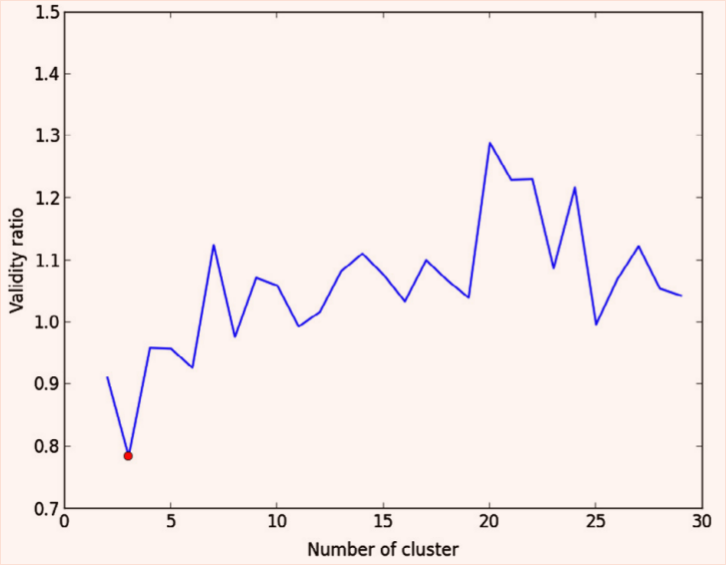
\includegraphics[scale=0.2]{Figures/MalignantOriginal}
    \caption*{(a) Original Result}
\end{minipage}%
\begin{minipage}[t]{0.5\linewidth}
    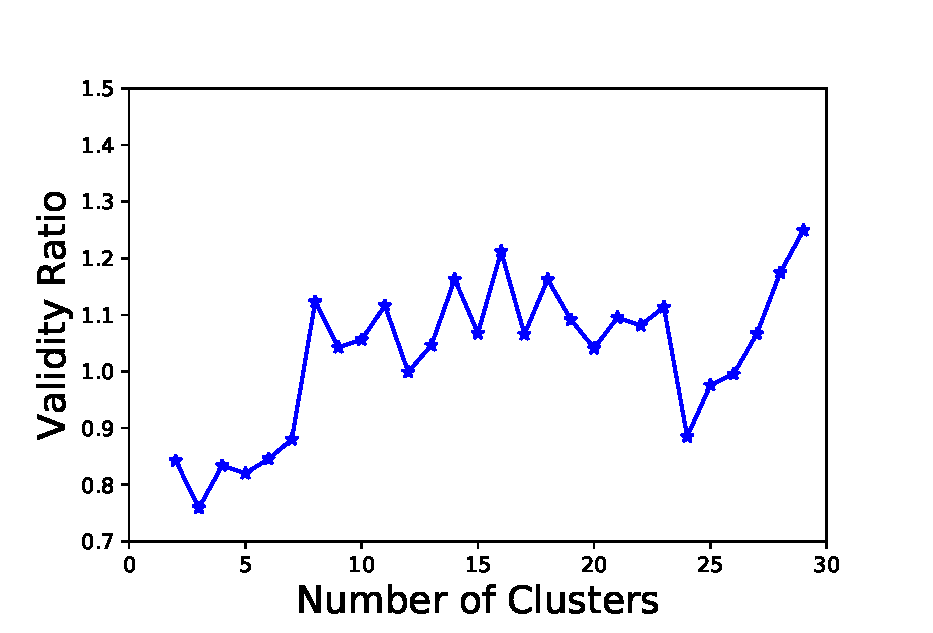
\includegraphics[scale=0.43]{Figures/Malignant_VR_K_AllX.eps}
    \caption*{(b) New Result}
\end{minipage} 
\end{figure}

\begin{block}{}
\begin{itemize}
\item Minimum value is achieved when K = 3.
\item Validity ratio is not same in both the results. Could be due to random initialization of cluster center in K-means.
\end{itemize} 
\end{block}
\end{frame}

\begin{frame}{New Results (Benign): Separate Normalization}
Instances of both the classes are normalized separately.
\begin{figure}[H]
\begin{minipage}[t]{0.5\linewidth}
    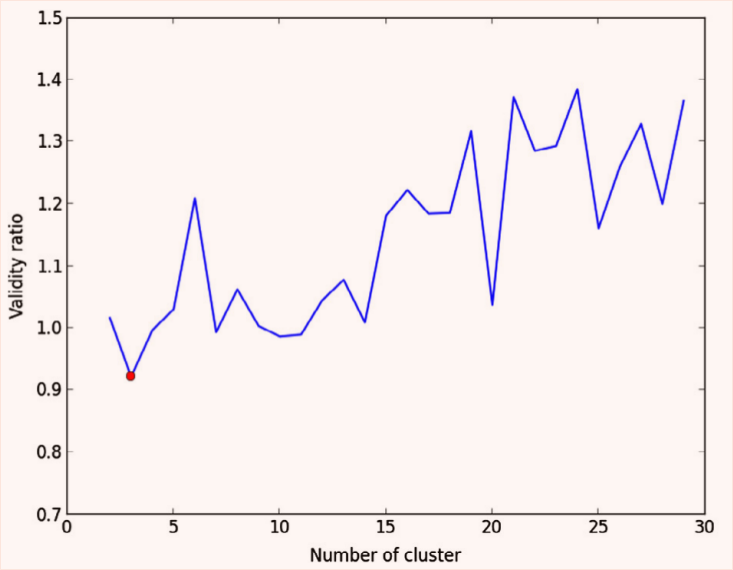
\includegraphics[scale=0.2]{Figures/BenignOriginal}
    \caption*{(a) Original Result}
\end{minipage}%
\begin{minipage}[t]{0.5\linewidth}
    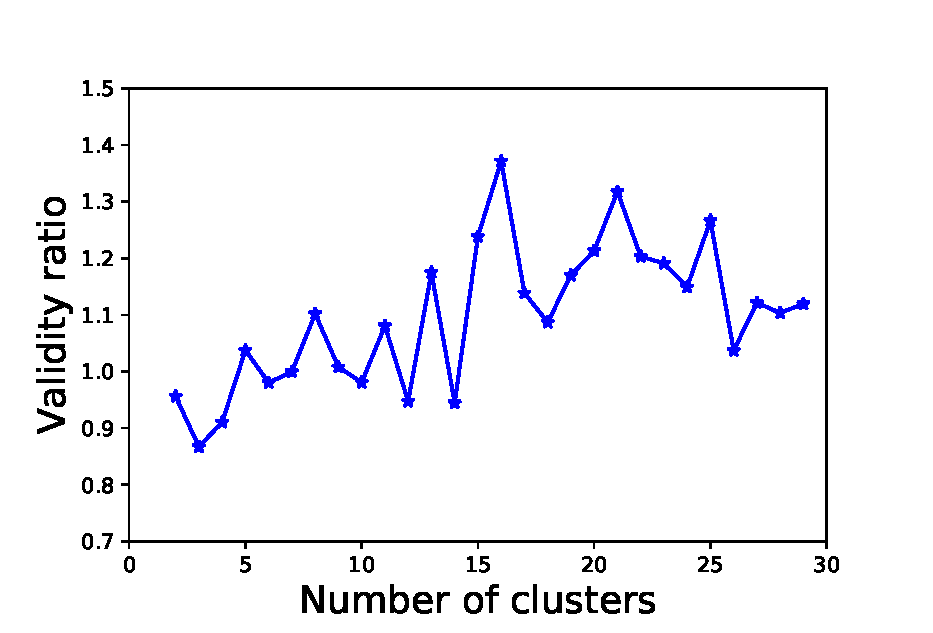
\includegraphics[scale=0.43]{Figures/Benign_VR_K_New.eps}
    \caption*{(b) New Result}
\end{minipage} 
\end{figure} 

\begin{block}{}
\begin{itemize}
\item Minimum value is achieved when K = 3.
\item Validity ratio is not same in both the results. Could be due to random initialization of cluster center in K-means.
\end{itemize} 
\end{block}
\end{frame}

\begin{frame}{New Results (Malignant): Separate Normalization}
Instances of both the classes are normalized separately.
\begin{figure}[H]
\begin{minipage}[t]{0.5\linewidth}
    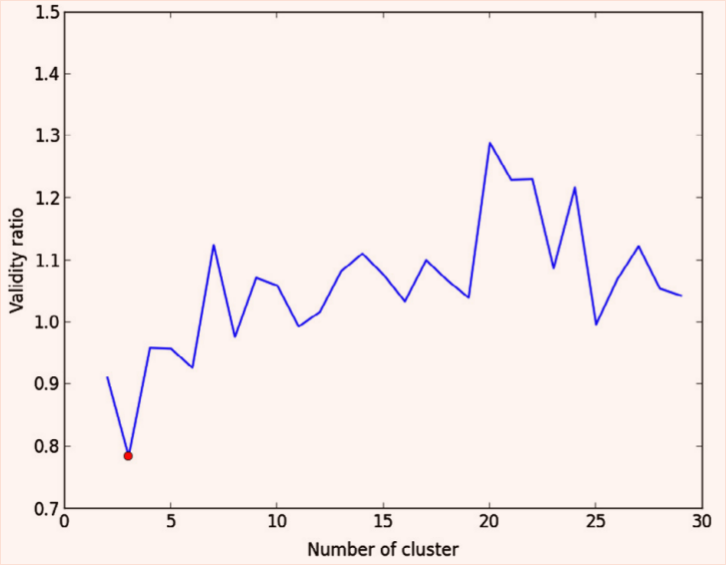
\includegraphics[scale=0.2]{Figures/MalignantOriginal}
    \caption*{(a) Original Result}
\end{minipage}%
\begin{minipage}[t]{0.5\linewidth}
    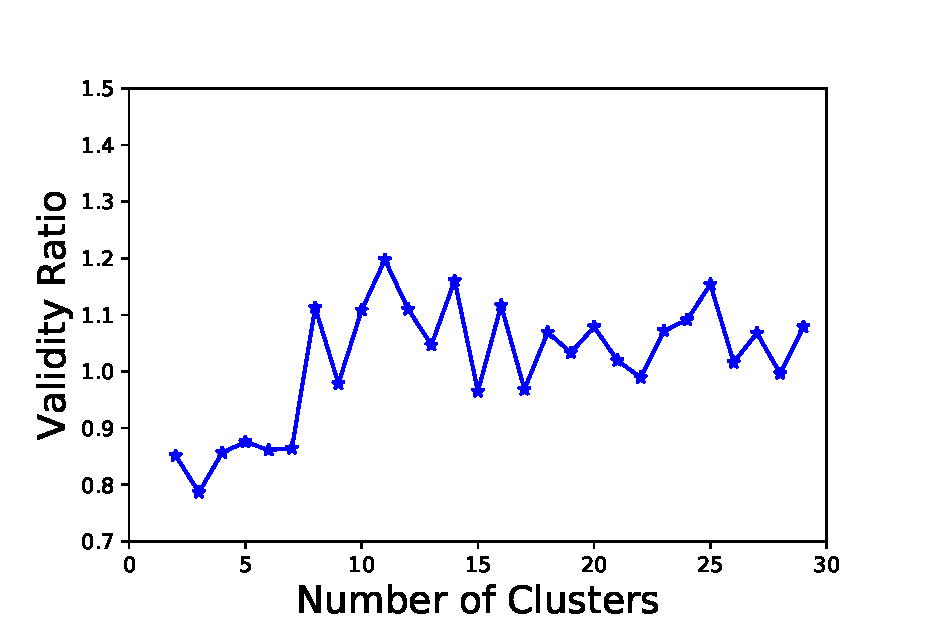
\includegraphics[scale=0.43]{Figures/Malignant_VR_K_New.eps}
    \caption*{(b) New Result}
\end{minipage} 
\end{figure}

\begin{block}{}
\begin{itemize}
\item Minimum value is achieved when K = 3.
\item All the other results are obtained from separate normalization.
\end{itemize} 
\end{block}
\end{frame}


\begin{frame}{New Results: Silhouette Value}
\begin{figure}[H]
\begin{minipage}[t]{0.5\linewidth}
    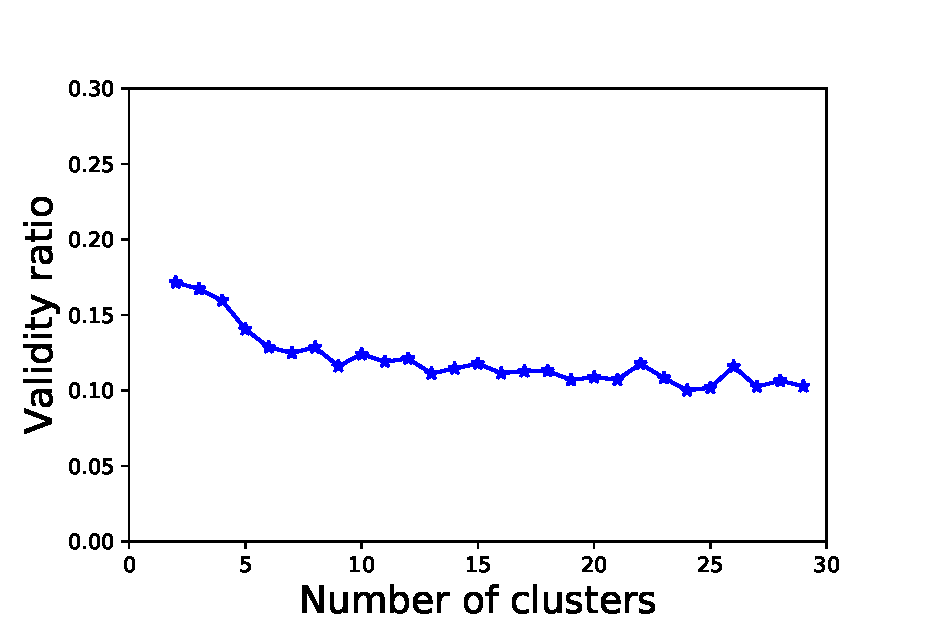
\includegraphics[scale=0.43]{Figures/Benign_VR_K_Sil.eps}
    \caption*{(a) Benign Tumor}
\end{minipage}%
\begin{minipage}[t]{0.5\linewidth}
    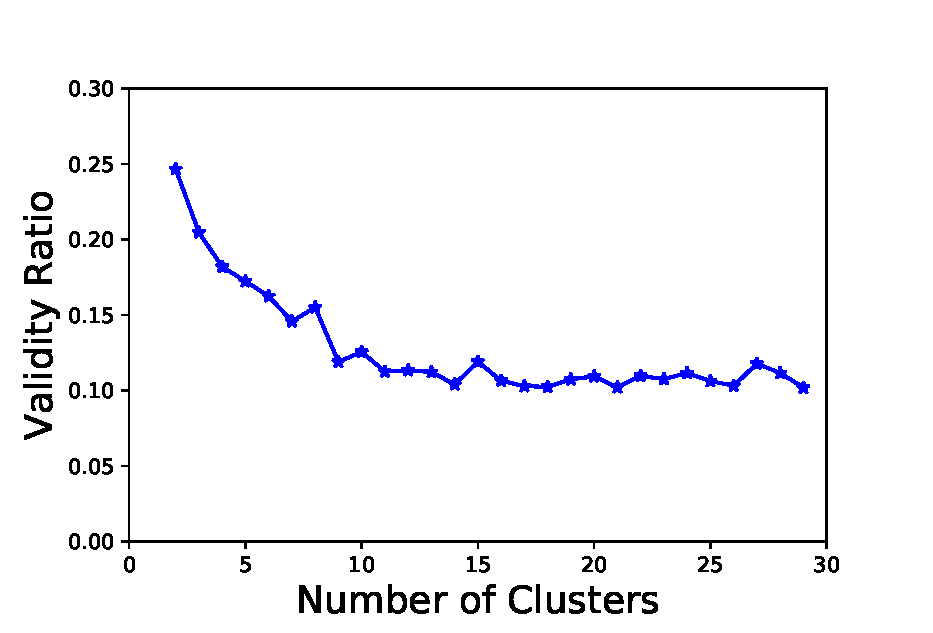
\includegraphics[scale=0.43]{Figures/Malignant_VR_K_Sil.eps}
    \caption*{(b) Malignant Tumor}
\end{minipage} 
\end{figure}

\begin{block}{}
\begin{itemize}
\item For both the classes maximum value is achieved when K = 2.
\item Different from results obtained using validity ration
\end{itemize} 
\end{block}
\end{frame}


\begin{frame}{Feature Extraction and SVM model}
\begin{itemize}
\item The six cluster centers give symbolic representation of the clusters. 
\item Six features are extracted using these six cluster centers.
\end{itemize}
\begin{align*}
f_c(X^i_j) &= \begin{cases}
    1 - \frac{|X_j^{\mu_c}-X_j^i|}{\max|X_j^{\mu_c}-X_j^n|},& \text{if } \min(X_j^n) \leq X_j^i \leq \max(X_j^n),\; \forall n \in S_c\\
    0,              & \text{otherwise}
\end{cases}\\ 
p_c &= \frac{1}{F} \sum_{j=1}^Ff_c(X_j^i),\;\; 1\leq c \leq K^m + K^b
\end{align*}

\vspace{0.5cm}
\alert{SVM model is built using the extracted features to diagnose breast cancer.}
\end{frame}


\section{Results}

\begin{frame}{Experimental Setup}
\begin{table}[]
\centering
\begin{tabular}{|l|l|}
\hline
Parameter          & Value                                                                                      \\ \hline
SVM penalty  (C)   & 0.1, 1, 10, 20, $\cdots$, 100                                                               \\
Kernels            & Linear and Sigmoid                                                                         \\
Cross Vaidation	   & 10-fold cross validation\\	
Performance metrics & Test accuracy, sensitivity, specificity and time \\
Programming Language & Python (Scikit) \\
Processor          & Intel Core i7 with 2.5 GHz processor                                                      \\ \hline
\end{tabular}
\end{table}
\end{frame}

\subsection{Linear Kernel}

\begin{frame}{Linear Kernel: Accuracy, Sensitivity and Specificity}
\alert{Y axis range is different in the figures}
\begin{figure}[H]
\begin{minipage}[t]{0.5\linewidth}
    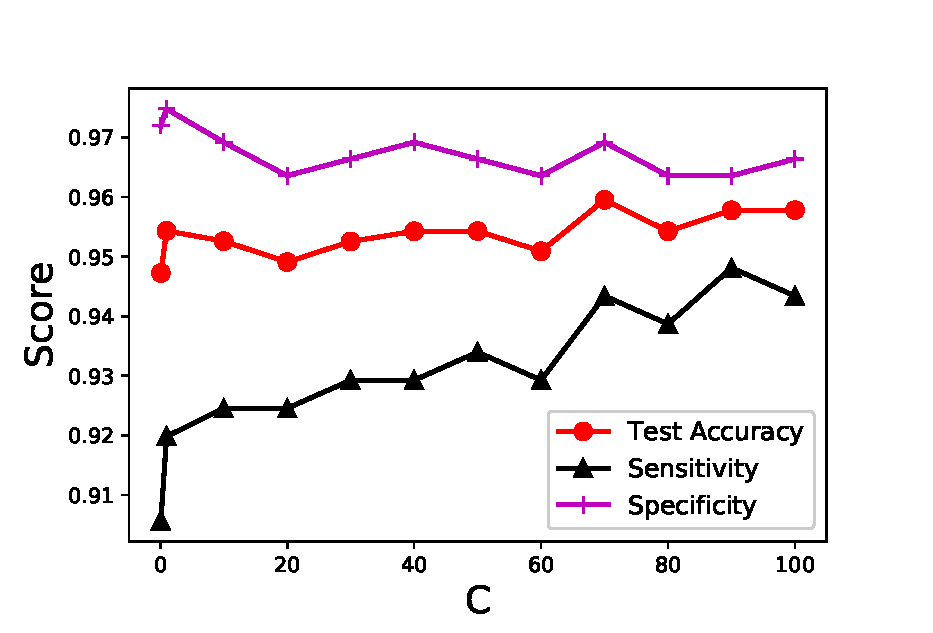
\includegraphics[scale=0.43]{Figures/SVM_Linear_Accuracy.eps}
    \caption*{(a) SVM}
\end{minipage}%
\begin{minipage}[t]{0.5\linewidth}
    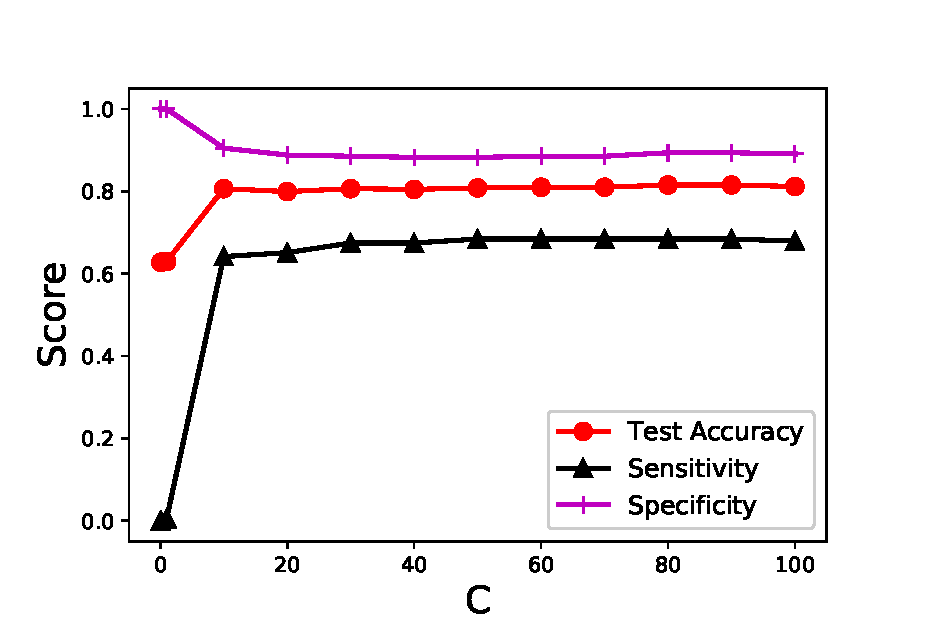
\includegraphics[scale=0.43]{Figures/KSVM_Linear_Accuracy.eps}
    \caption*{(b) KSVM}
\end{minipage} 
\end{figure}

\begin{block}{}
\begin{itemize}
\item Highest accuracy for SVM is 0.96 at C = 70.
\item Highest accuracy for KSVM is 0.81 at C = 80.
\end{itemize}
\end{block}
\end{frame}

\begin{frame}{Linear Kernel: Confusion Matrix}
\begin{figure}[H]
\begin{minipage}[t]{0.5\linewidth}
    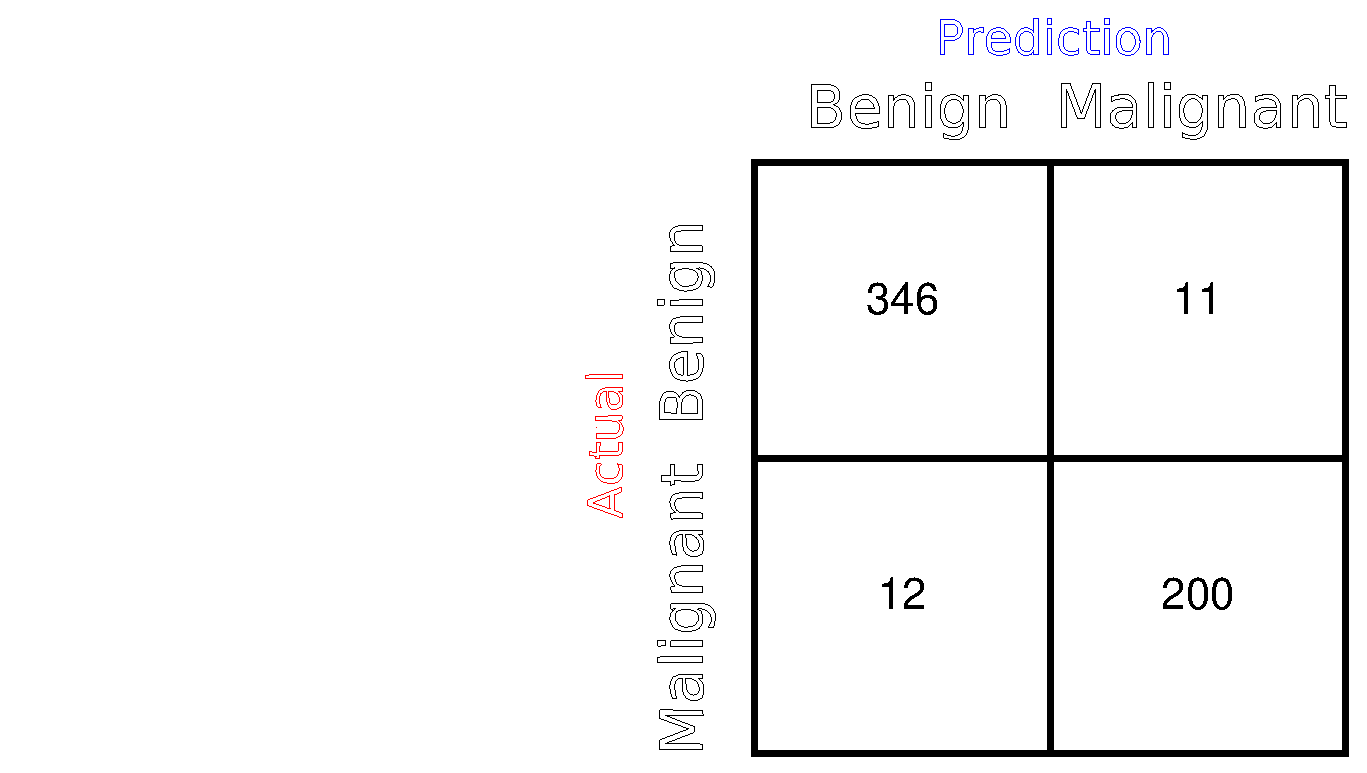
\includegraphics[trim={9cm 0cm 0cm 0cm},clip,scale=0.43]{Figures/SVM_Linear_CM.eps}
    \caption*{(a) SVM (C = 70)}
\end{minipage}%
\begin{minipage}[t]{0.5\linewidth}
    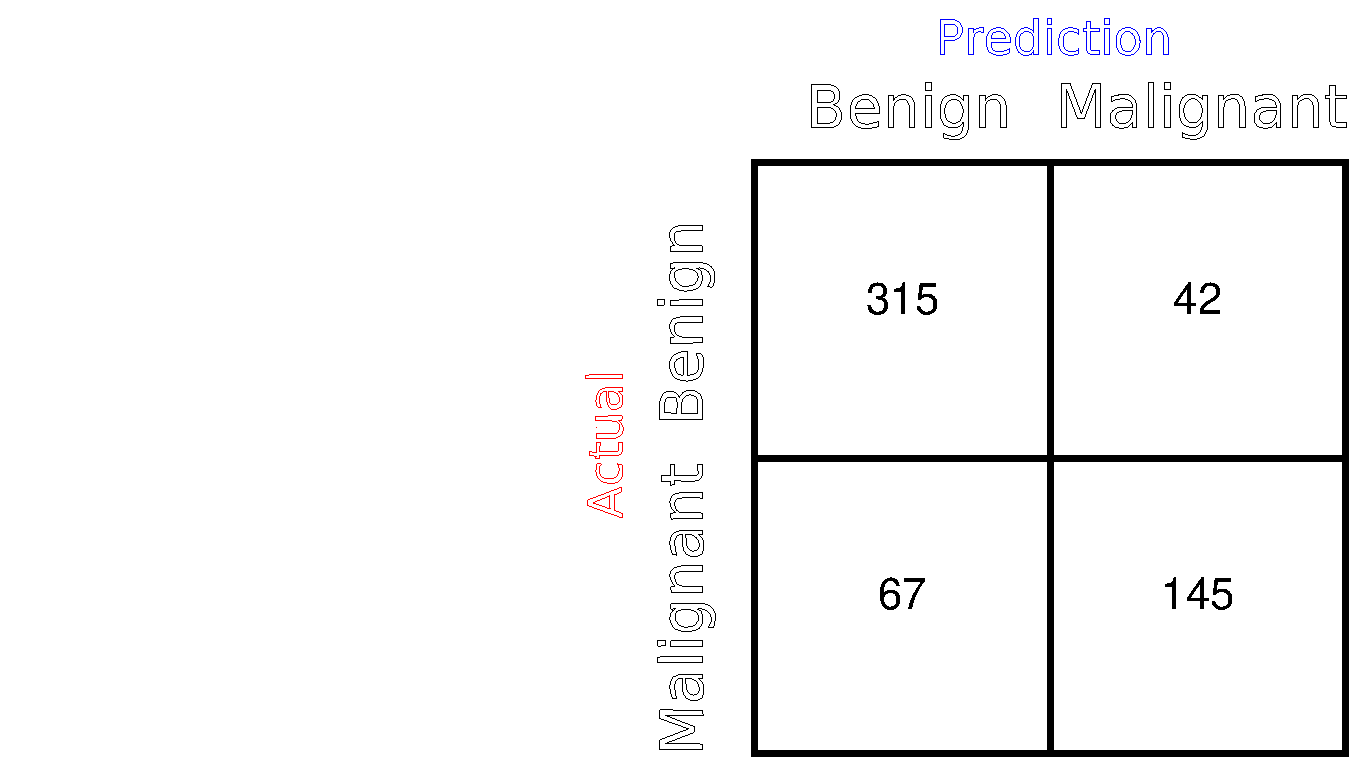
\includegraphics[trim={9cm 0cm 0cm 0cm},clip,scale=0.43]{Figures/KSVM_Linear_CM.eps}
    \caption*{(b) KSVM (C = 80)}
\end{minipage} 
\end{figure}
\end{frame}

\begin{frame}{Linear Kernel: Computation Time}
\begin{table}[]
\label{my-label}
\begin{tabular}{|l|l|l||l|l|l|}
\hline
C   & \begin{tabular}[c]{@{}l@{}}SVM Time\\(in sec)\end{tabular} & \begin{tabular}[c]{@{}l@{}}KSVM Time \\ (in sec)\end{tabular} & C   & \begin{tabular}[c]{@{}l@{}}SVM Time \\(in sec)\end{tabular} & \begin{tabular}[c]{@{}l@{}}KSVM Time\\ (in sec)\end{tabular} \\ \hline
0.1 & 2.8                                                                      & 0.03                                                                     & 50  & 94.5                                                                    & 0.05                                                                     \\
1   & 11.3                                                                     & 0.04                                                                     & 60  & 67.8                                                                    & 0.06                                                                     \\
10  & 47.9                                                                     & 0.04                                                                     & 70  & 71.8                                                                    & 0.05                                                                     \\
20  & 49.1                                                                     & 0.05                                                                     & 80  & 71.34                                                                   & 0.06                                                                     \\
30  & 64.3                                                                     & 0.04                                                                     & 90  & 74.9                                                                    & 0.06                                                                     \\
40  & 79.2                                                                     & 0.05                                                                     & 100 & 75.91                                                                   & 0.07                                                                    \\ \hline
\end{tabular}
\end{table}
As expected, less computation time  is required in KSVM than SVM.
\end{frame}

\subsection{Sigmoid Kernel}
\begin{frame}{Sigmoid Kernel: Accuracy, Sensitivity and Specificity}
\begin{figure}[H]
\begin{minipage}[t]{0.5\linewidth}
    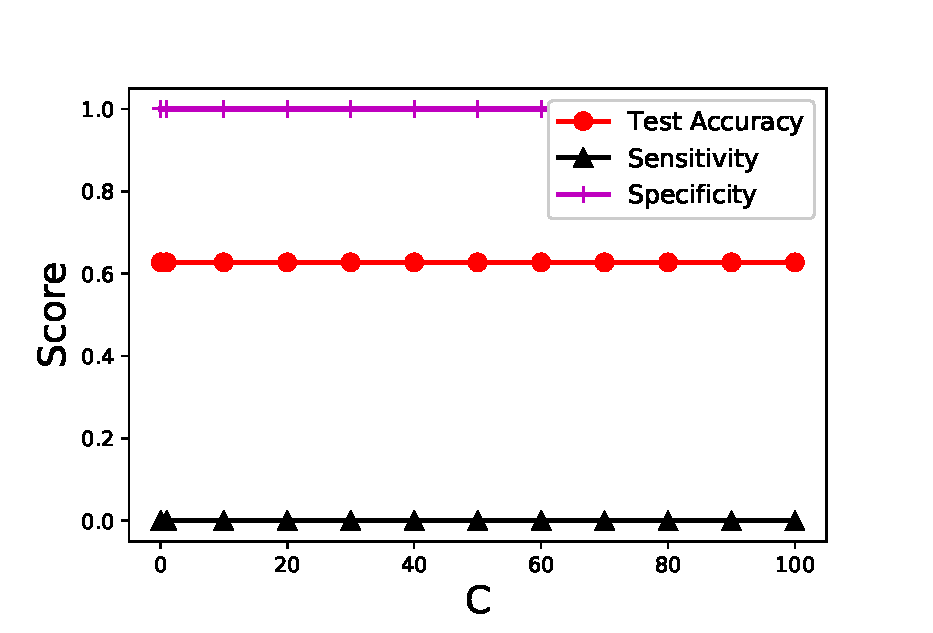
\includegraphics[scale=0.43]{Figures/SVM_Sigmoid_Accuracy.eps}
    \caption*{(a) SVM}
\end{minipage}%
\begin{minipage}[t]{0.5\linewidth}
    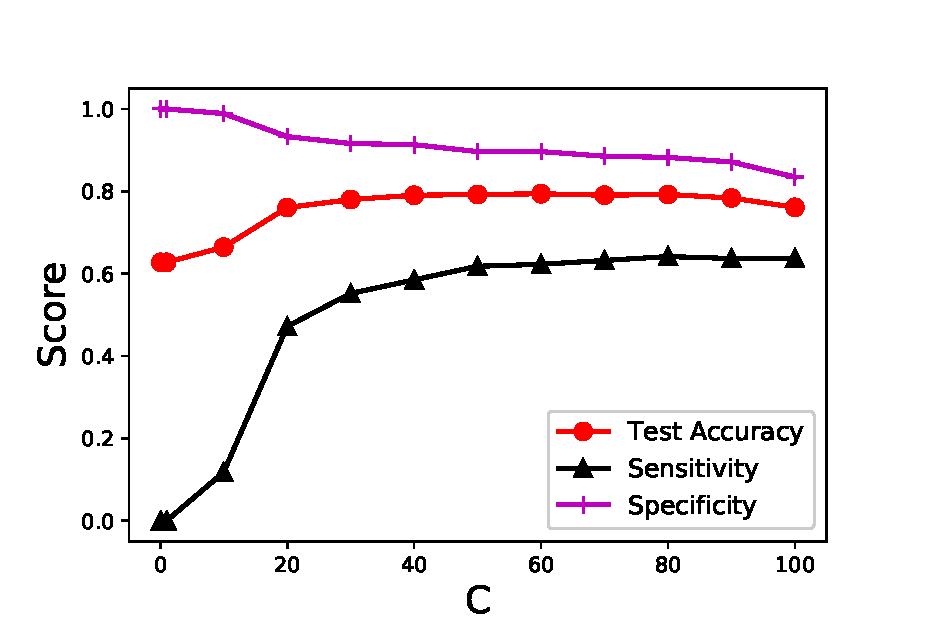
\includegraphics[scale=0.43]{Figures/KSVM_Sigmoid_Accuracy.eps}
    \caption*{(b) KSVM}
\end{minipage} 
\end{figure}

\begin{block}{}
\begin{itemize}
\item Highest accuracy for SVM is 0.63 at all C and gamma value.
\item Highest accuracy for KSVM is 0.79 at C = 80 and gamma = 0.167.
\item Accuracy for KSVM reported in paper is 0.97 \alert{(C value and gamma value are not mentioned)}.
\end{itemize}
\end{block}
\end{frame}

\begin{frame}{Sigmoid Kernel: Confusion Matrix}
\begin{figure}[H]
\begin{minipage}[t]{0.5\linewidth}
    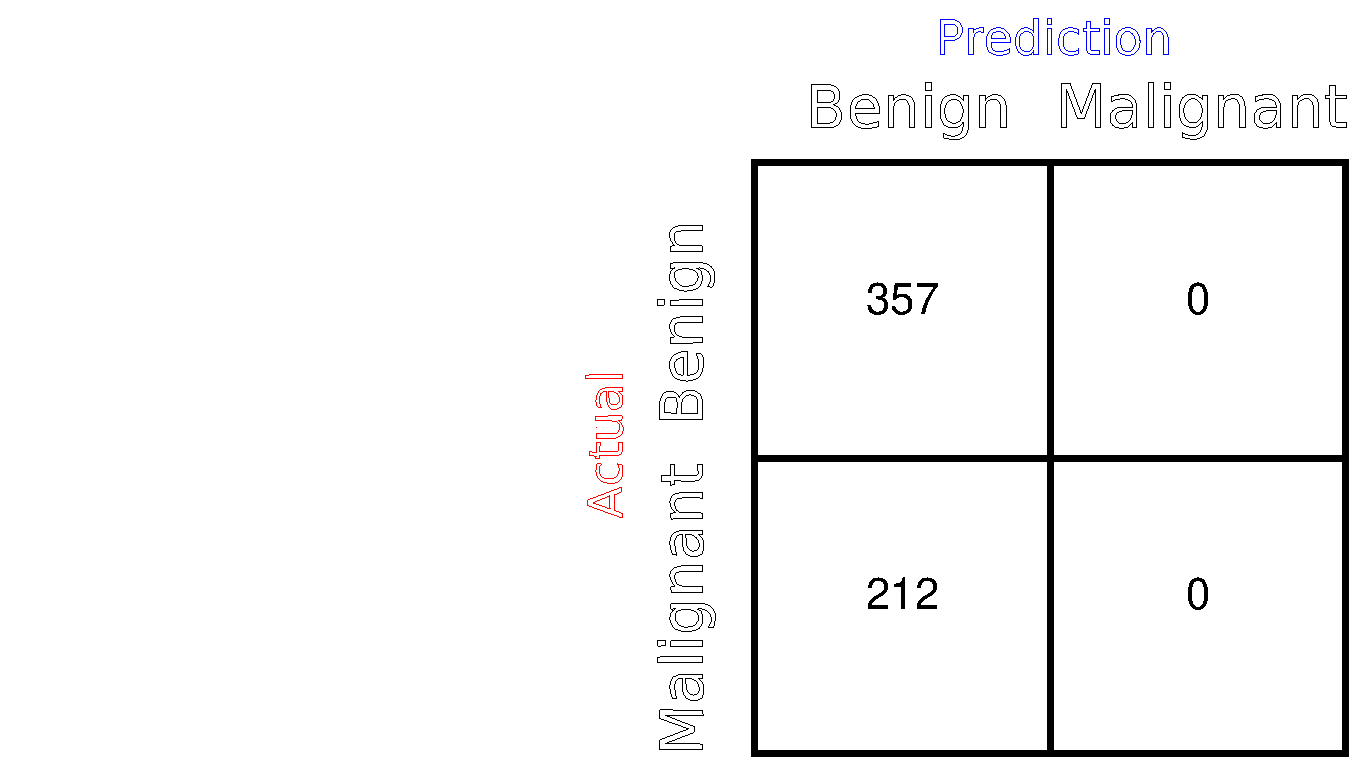
\includegraphics[trim={9cm 0cm 0cm 0cm},clip,scale=0.43]{Figures/SVM_Sigmoid_CM.eps}
    \caption*{(a) SVM (All C)}
\end{minipage}%
\begin{minipage}[t]{0.5\linewidth}
    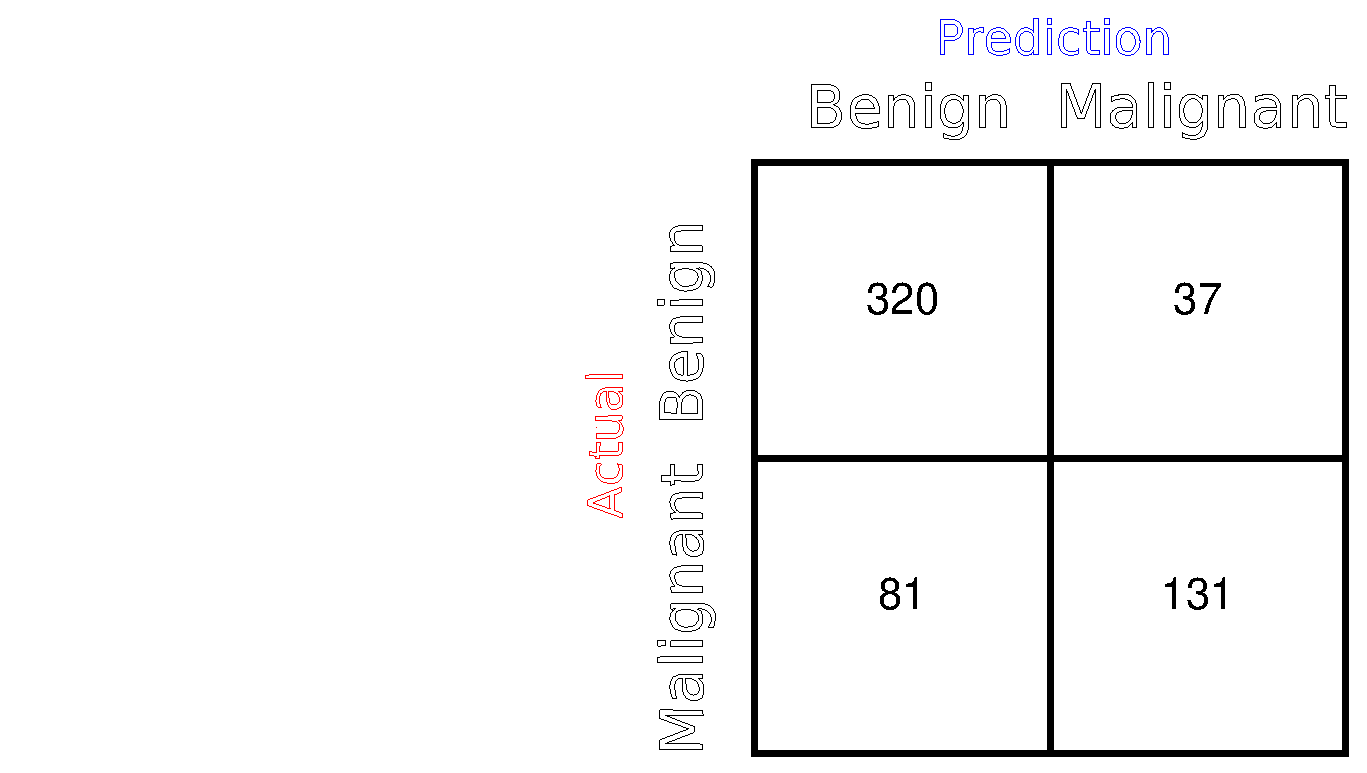
\includegraphics[trim={9cm 0cm 0cm 0cm},clip,scale=0.43]{Figures/KSVM_Sigmoid_CM.eps}
    \caption*{(b) KSVM (C = 80)}
\end{minipage} 
\end{figure}
\end{frame}


\section{Paper Summary}
\begin{frame}{Paper Summary}
\begin{table}[]
\centering
\begin{tabular}{|l|l|l|}
\hline
Prediction           & Feature Selection                                                    & ML Algorithm                                                                                                     \\ \hline \hline
Breast Cancer        & F1-Score                                                             & SVM                                                                                                              \\ \hline
Diabetes             & \begin{tabular}[c]{@{}l@{}}Information Gain\\ and SMOTE\end{tabular} & \begin{tabular}[c]{@{}l@{}}Decision Trees,\\ Logistic Regression,\\ Naive Bayes and\\ Random Forest\end{tabular} \\ \hline
Hospital Readmission & Oversampling                                                         & \begin{tabular}[c]{@{}l@{}}Particle Swarm \\ Optimization based SVM\end{tabular}                                 \\ \hline
Breast Cancer        & K-Means                                                              & SVM                                                                                                             \\ \hline
\end{tabular}
\end{table}
\end{frame}

\begin{frame}[allowframebreaks]
\nocite{*}
\printbibliography[heading=none]
        \frametitle{References}
\end{frame} 
\end{document}